%% State Space Modelling of Dynamic Systems
%% Normal Canonical Form
\def\FileDate{98/11/03}
\def\FileVersion{1.0}
% ----------------------------------------------------------------
% Notes pages *********************************************************
% ----------------------------------------------------------------

In the previous lecture we examined the companion form of a
state-space model which allows the direct transformation of a transfer
function into state space form. In this lecture we examine three
other ``canonical forms'' the \emph{controller canonical form},
the \emph{observer canonical form} and the ``\emph{normal form}''. 


\section*{Controller Canonical Form}
If one defines a transfer function in \Matlab{}, e.g. as shown in
\sref{slide:l5s5}, the result of converting the system into
state-space form is rather surprisingly not the companion form we
have seen before. Instead, the result is what is known as the
\emph{Controller Canonical Form}. This is still a companion form
because the coefficients of the $\mathbf{A}$ and $\mathbf{C}$
matrices are the coefficients of the transfer function's
denominator and numerator polynomials.
\begin{slide}\label{slide:l5s5}\heading{A Little \Matlab{}}
Let \[ G(s)
=\frac{Y(s)}{U(s)} = \frac{s^2 + 7s + 2 }{s^3 + 9s^2 + 26s + 24}\]
\begin{verbatim}
>> num=[1, 7, 2]; den=[1, 9, 26 24];
>> [A,B,C,D]=tf2ss(num,den);
\end{verbatim}
Result:
\begin{eqnarray*}
\dot{\mathbf{x}} & = &\left[\begin{array}{ccc}
  -9 & -26 & -24  \\
  1 & 0 & 0  \\
  0 & 1  & 0
 \end{array}\right]\mathbf{x}+\left[\begin{array}{c}
  1 \\
  0 \\
  0
\end{array}\right]u\\
y & = & [1,\ 7,\ 2] \mathbf{x}.\end{eqnarray*}
\end{slide}
The controller canonical form is simply obtained by re-ordering
the phase variables as shown in \sref{slide:l5s6},
\sref{slide:l5s6-2} and \sref{slide:l5s7}. The general form of the
controller canonical state-space model is as shown in
\sref{slide:l5s8}.
\begin{slide}
\label{slide:l5s6} \heading{Companion Form}
\begin{eqnarray*} \left[\begin{array}{c}
  \dot{x}_{1} \\
  \dot{x}_{2} \\
  \vdots \\
  \dot{x}_{n-1} \\
  \dot{x}_n
\end{array}\right] &=& \left[\begin{array}{ccccc}
  0 & 1 & 0 & \cdots & 0 \\
  0 & 0 & 1 & \cdots & 0 \\
  \vdots & \vdots & \vdots & \ddots & \vdots \\
  0 & 0 & 0 & \cdots & 1 \\
  -a_{0} & -a_{1} & -a_{2} & \cdots & -a_{n-1}
\end{array}\right]\left[\begin{array}{c}
  {x}_{1} \\
  {x}_{2} \\
  \vdots \\
  {x}_{n-1} \\
  {x}_{n}
\end{array}\right]+\left[\begin{array}{c}
  0 \\
  0 \\
  \vdots \\
  0 \\
  1
\end{array}\right]u\\
y & = & [b_0,\ b_1,\ \dots,\ b_{n-2}, b_{n-1}][
  {x}_{1},\
  {x}_{2},\
  \ldots,\
  {x}_{n-1},\
  {x}_{n}]^T
\end{eqnarray*}
\end{slide}
\begin{slide}\label{slide:l5s6-2}
\heading{Controller canonical form: Re-number States}

\begin{eqnarray*} \left[\begin{array}{c}
  \dot{x}_{n} \\
  \dot{x}_{n-1} \\
  \vdots \\
  \dot{x}_{2} \\
  \dot{x}_{1}
\end{array}\right] &=& \left[\begin{array}{ccccc}
  0 & 1 & 0 & \cdots & 0 \\
  0 & 0 & 1 & \cdots & 0 \\
  \vdots & \vdots & \vdots & \ddots & \vdots \\
  0 & 0 & 0 & \cdots & 1 \\
  -a_{0} & -a_{1} & -a_{2} & \cdots & -a_{n-1}
\end{array}\right]\left[\begin{array}{c}
  {x}_{n} \\
  {x}_{n-1} \\
  \vdots \\
  {x}_{2} \\
  {x}_{1}
\end{array}\right]+\left[\begin{array}{c}
  0 \\
  0 \\
  \vdots \\
  0 \\
  1
\end{array}\right]u\\ y & = & [b_0,\ b_1,\ \dots,\ b_{n-2}, b_{n-1}]
\left[
  {x}_{n},\
  {x}_{n-1},\
  \ldots,\
  {x}_{2},\
  {x}_{1}
\right]^T
\end{eqnarray*}
\end{slide}
\begin{slide}\label{slide:l5s7}
\heading{Controller canonical form: Re-Ordered States}

\begin{eqnarray*} \left[\begin{array}{c}
  \dot{x}_{1} \\
  \dot{x}_{2} \\
  \vdots \\
  \dot{x}_{n-1} \\
  \dot{x}_{n}
\end{array}\right] &=& \left[\begin{array}{ccccc}
 -a_{n-1} & -a_{n-2} & \cdots & -a_{1} & -a_{0} \\
   1 & 0 & \cdots & 0 & 0 \\
  0 & 1 & \cdots & 0 & 0 \\
  \vdots & \vdots & \ddots & \vdots & \vdots \\
  0 & 0 & \cdots & 1 & 0
\end{array}\right]\left[\begin{array}{c}
  {x}_{1} \\
  {x}_{2} \\
  \vdots \\
  {x}_{n-1} \\
  {x}_{n}
\end{array}\right]+\left[\begin{array}{c}
  1 \\
  0 \\
  \vdots \\
  0 \\
  0
\end{array}\right]u\\ y & = & [b_{n-1},\ b_{n-2},\ \dots,\ b_{1}, b_{0}]
\left[
  {x}_{1},\
  {x}_{2},\
  \ldots,\
  {x}_{n-1},\
  {x}_{n}
\right]^T
\end{eqnarray*}
\end{slide}
\begin{slide}
\label{slide:l5s8} \heading{Controller Canonical Form: Block
Diagram} \resizebox{300pt}{!}{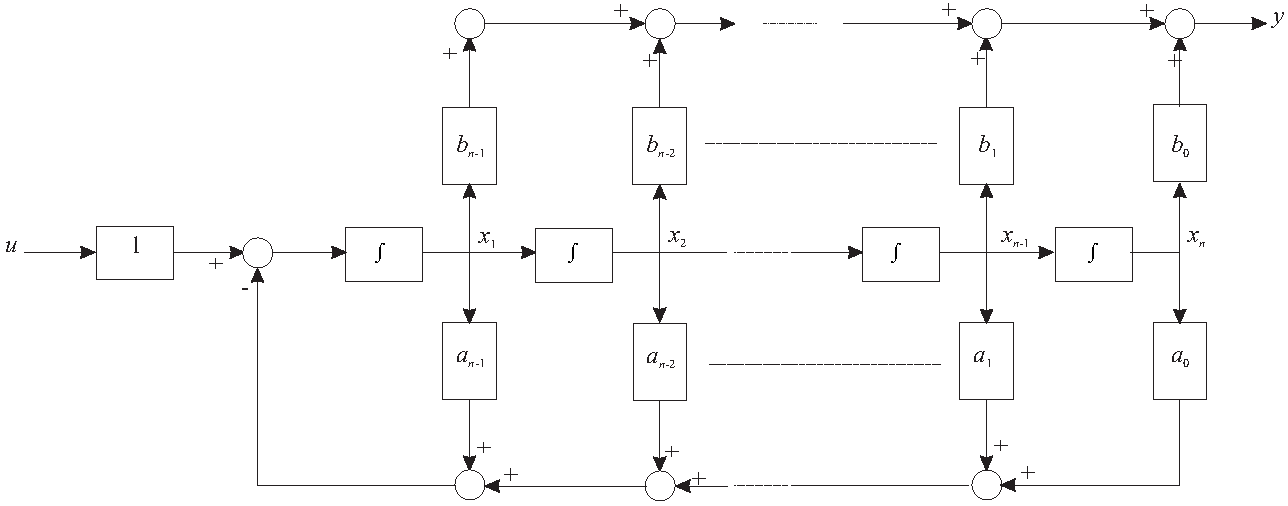
\includegraphics{pictures/ccanon.pdf}}
\end{slide}

\section*{Observer Canonical Form}
The observer canonical form is the "dual" of the controller
canonical form. The state equations are shown in
\sref{slide:l5s9}. Note that the $\mathbf{A}$ matrix is the
transpose of the controller canonical form and that $\mathbf{b}$
and $\mathbf{c}$ are the transposes of the $\mathbf{c}$ and
$\mathbf{b}$ matrices, respectively, of the controller canonical
form.
\begin{slide} \label{slide:l5s9} \heading{Observer Canonical Form}
\begin{eqnarray*} \left[\begin{array}{c}
  \dot{x}_{n} \\
  \dot{x}_{n-1} \\
  \vdots \\
  \dot{x}_{2} \\
  \dot{x}_{1}
\end{array}\right] &=& \left[\begin{array}{ccccc}
 -a_{n-1} & 1 & 0 & \cdots & 0 \\
 -a_{n-2} & 0 & 1 & \cdots & 0 \\
 -a_{n-3} & 0 & 0 & \cdots & 0 \\
  \vdots & \vdots & \vdots & \ddots & \vdots \\
 -a_{1} & 0 & \cdots & 0 & 1 \\
 -a_{0} & 0 & \cdots & 0 & 0
\end{array}\right]\left[\begin{array}{c}
  {x}_{1} \\
  {x}_{2} \\
  {x}_{3} \\
  \vdots \\
  {x}_{n-1} \\
  {x}_{n}
\end{array}\right]+\left[\begin{array}{c}
  b_{n-1} \\
  b_{n-2} \\
  b_{n-3} \\
  \vdots \\
  b_{1} \\
  b_0
\end{array}\right]u\\ y & = & [1,\ 0,\ 0,\ \ldots, 0]\left[
  {x}_{1},\
  {x}_{2},\
  \ldots,\
  {x}_{n-1},\
  {x}_{n}
\right]^T
\end{eqnarray*}
\end{slide}
\begin{slide}
\label{slide:l5s} \heading{Observer Canonical Form: Block Diagram}
\resizebox{300pt}{!}{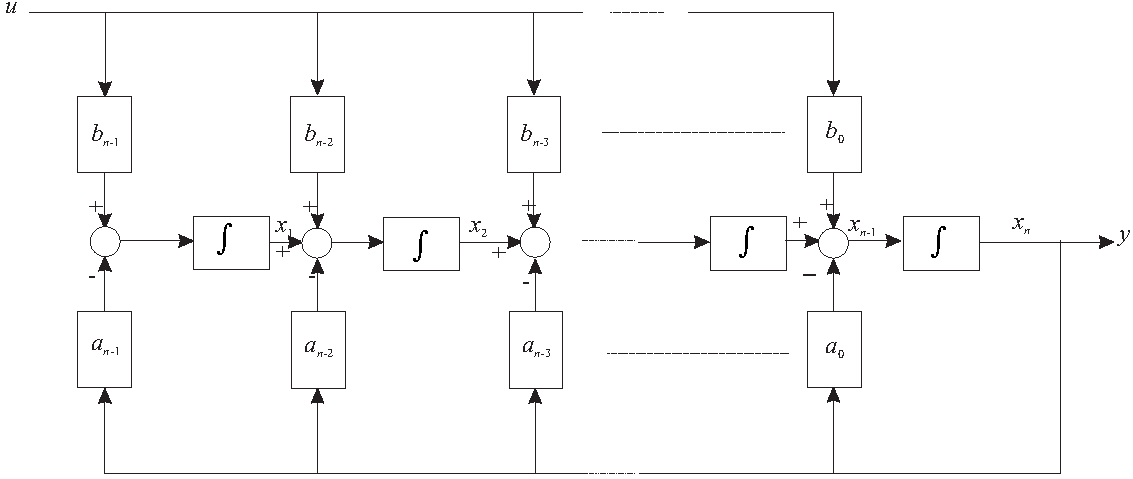
\includegraphics{pictures/ocanon.pdf}}
\end{slide}

\section*{Examples of Companion Forms}
The system with transfer function
\[G(s)=\frac{Y(s)}{U(s)}=\frac{2s^3 + 16s^2 + 30s + 8}{s^3 + 7s^2 + 10s}\]
was found, in the last lecture, to have companion form
\begin{eqnarray*}\mathbf{A} & = & \left[\begin{array}{ccc}
  0 & 1 & 0 \\
  0 & 0 & 1 \\
  0 & -10 & -7
\end{array}\right]\ \mathbf{B}=\left[\begin{array}{c}
  0 \\
  0 \\
  1
\end{array}\right]\\ \mathbf{C} & = & \left[\begin{array}{ccc}
  8 & 10 & 2
\end{array}\right]\ \mathbf{D}=\left[2\right]\end{eqnarray*}
The controller canonical form is obtained by re-ordering the state
variables:
\begin{eqnarray*}\mathbf{A} & = & \left[\begin{array}{ccc}
  -7 & -10 & 0 \\
  1 & 0 & 0 \\
  0 & 1 & 0
\end{array}\right]\ \mathbf{B}=\left[\begin{array}{c}
  1 \\
  0 \\
  0
\end{array}\right]\\ \mathbf{C} & = & \left[\begin{array}{ccc}
  2 & 8 & 10
\end{array}\right]\ \mathbf{D}=\left[2\right]\end{eqnarray*}
and the observable canonical form is obtained by transposing the
$\mathbf{A}$ matrix and letting $\mathbf{B} = \mathbf{C}^T$ and
$\mathbf{C}=\mathbf{B}^T$.
\begin{eqnarray*}\mathbf{A} & = & \left[\begin{array}{ccc}
  -7 & 1 & 0 \\
  -10 & 0 & 1 \\
  0 & 0 & 0
\end{array}\right]\ \mathbf{B}=\left[\begin{array}{c}
  2 \\
  8 \\
  10
\end{array}\right]\\ \mathbf{C} & = & \left[\begin{array}{ccc}
  1 & 0 & 0
\end{array}\right]\ \mathbf{D}=\left[2\right]\end{eqnarray*}
\begin{slide}\label{slide:l5s10}
\heading{\Matlab{} Code for Example}
\begin{verbatim}
>> num = [2, 16, 30, 8]; den = [1, 7, 10, 0];
>> G = tf(num,den);
>> Gcc = ss(G);
>> [Acc,Bcc,Ccc,Dcc]=ssdata(Gcc);
\end{verbatim}
The resulting variables \verb|A|, \verb|B|, \verb|C|, and \verb|D|
are in controller canonical form.
\begin{verbatim}
>> Goc = ss(Acc',Ccc',Bcc',Dcc);
\end{verbatim}
will create the observer canonical form.
\end{slide}
\begin{slide}\label{slide:15s10a}
\heading{$\ldots$ Companion Form}
To obtain the companion form,
some \Matlab{} trickery is needed to re-order the controller
canonical state matrices:
\begin{verbatim}
>> [n,m]=size(Acc); % n = m = 3 for the example
>> Acf = Acc(n:-1:1,n:-1:1);
>> Bcf = Bcc(n:-1:1,:); 
>> Ccf = Ccc(:,n:-1:1);
>> Dcf = Dcc;
\end{verbatim}
The companion form is then created from the reordered matrices.
\begin{verbatim}
>> Gcf = ss(Acf,Bcf,Ccf,Dcf);
\end{verbatim}
\end{slide}
\begin{slide}\label{slide:l5s11}
\heading{\emph{All Forms} Represent the Same Transfer Function!}
\begin{verbatim}
>> G1 = tf(Gcf) % Companion form
Transfer function:
2 s^3 + 16 s^2 + 30 s + 8
-------------------------
   s^3 + 7 s^2 + 10 s
>> G2 = tf(Gcc) % Controller Canonical form
ditto!
>> G3 = tf(Goc) % Observer Canonical Form
ditto!
\end{verbatim}
\end{slide}
We now consider one
final canonical form, the so-called ``normal'' or ``parallel''
form.

\section*{Normal Canonical Form}
The normal form of
a state-space model isolates the characteristic values, also
called the eigen values, or system poles, of the system.

If all the poles of a system are real and distinct then the
transfer function may be written as a partial fraction expansion
\[ G(s) = \frac{Y(s)}{U(s)} = \left\{\frac{r_1}{s-p_1} +
\frac{r_2}{s-p_2} + \cdots + \frac{r_n}{s-p_n} + d\right\}
\]
we can develop a state-space model for each term:
\[Y(s)=\frac{r_i}{s-p_i}U(s).\]
\begin{eqnarray*}
(s-p_i)Y(s) & = & r_i U(s)\\ \frac{d}{dt}y(t)-p_i y(t) &=& r_i
u(t).\end{eqnarray*} If we let $x_i(t) = y(t)$ then
\begin{eqnarray*}
\dot{x}_i &=& p_i x_i + r_i u \\ y &=& x_i
\end{eqnarray*}
Thus, each partial fraction term may be represented by the block
diagram shown in \sref{slide:l6s1}.
\begin{slide}\label{slide:l6s1}
\heading{State-Space Model of $\frac{r_i}{s-p_i}$}
\begin{eqnarray*}
\dot{x}_i &=& p_i x_i + r_i u \\ y &=& x_i
\end{eqnarray*}
\resizebox{300pt}{!}{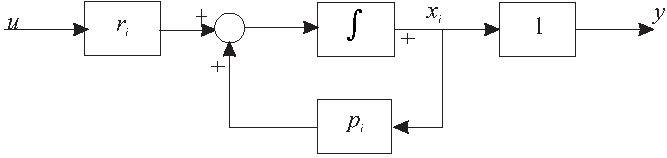
\includegraphics{pictures/sspole.pdf}}
\end{slide}
Thus, the total state-space model of the system is simply the sum
of such terms as shown in \sref{slide:l6s2}.
\begin{slide}\label{slide:l6s2}
\heading{Normal Canonical Form: Block Diagram}
\resizebox{300pt}{!}{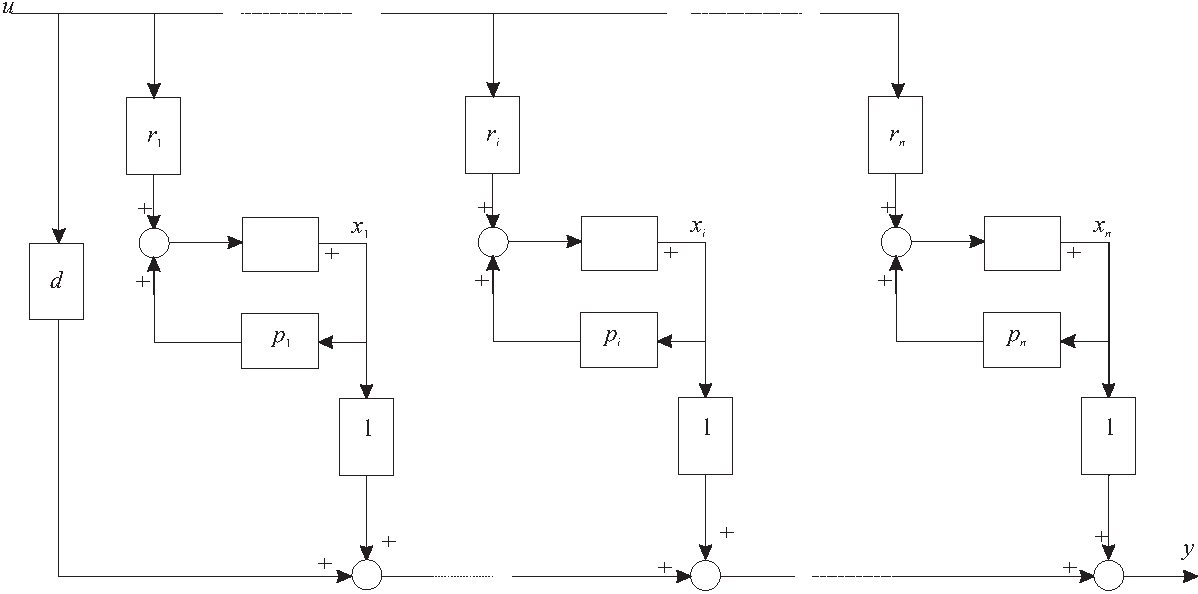
\includegraphics{pictures/normalcan.pdf}}
\end{slide}

Therefore the state space model for the whole system is as shown
in \sref{slide:l6s3}.
\begin{slide}\label{slide:l6s3}
\heading{Normal Observable Canonical State Space Model}
\begin{eqnarray*} \mathbf{\dot{x}}&=&\left[\begin{array}{ccccc}
  p_1 & 0 & 0 & \cdots & 0 \\
  0 & p_2 & 0 & \cdots & 0 \\
  0 & 0 & p_3 & \cdots & 0 \\
  \vdots & \vdots & \vdots & \ddots & \vdots \\
  0 & 0 & 0 & \cdots & p_n
\end{array}\right] \mathbf{x} + \left[\begin{array}{c}
  r_1 \\
  r_2 \\
  r_3 \\
  \vdots \\
  r_n
\end{array}\right] u\\ y &=& \left[1,\ 1,\ 1,\ \ldots,\ 1\right] \mathbf{x} + d u
\end{eqnarray*}
 \end{slide}

Note that the residues of the partial fraction expansion $r_1,\
r_2,\ \ldots,\ r_n$ have been allocated to the input side of the
block diagram and therefore to the input matrix in the state space
model. This model, in which all the elements of the output matrix
are unity, is called the ``\emph{Normal Observable Canonical
Form}''. It would be equally valid to allocate the residues to the
output matrix, leaving the elements of the input matrix as unity,
this would be the ``\emph{Normal Controllable Canonical Form}''
illustrated in \sref{slide:l6s3b}.

\begin{slide}\label{slide:l6s3b}
\heading{Normal Controllable Canonical State Space Model}
\begin{eqnarray*} \mathbf{\dot{x}}&=&\left[\begin{array}{ccccc}
  p_1 & 0 & 0 & \cdots & 0 \\
  0 & p_2 & 0 & \cdots & 0 \\
  0 & 0 & p_3 & \cdots & 0 \\
  \vdots & \vdots & \vdots & \ddots & \vdots \\
  0 & 0 & 0 & \cdots & p_n
\end{array}\right] \mathbf{x} + \left[\begin{array}{c}
  1 \\
  1 \\
  1 \\
  \vdots \\
  1
\end{array}\right] u\\ y &=& \left[r_1,\ r_2,\ r_3,\ \ldots,\ r_n\right] \mathbf{x} + d u
\end{eqnarray*}
 \end{slide}

The most important property of the normal canonical model is that
the $\mathbf{A}$ matrix is diagonal and that the elements on the
diagonal are the eigenvalues of the system matrix. If you form the
system transition matrix for this system each state response is
simply of the form $r_i e^{p_i t}$, that is each state response is
equal to the corresponding mode response\footnote{The proof is
left as an exercise.}.

\subsection*{Example}
For the system examined earlier
\begin{eqnarray*}
G(s) &=& \frac{2s^3 + 16s^2 + 30s + 8}{s^3 + 7s^2 + 10s} \\
 &=&
\frac{2s^2 + 10s + 8}{s^3 + 7s^2 + 10s} + 2 \\
 &=& \frac{2s^2 + 10s + 8}{s(s+2)(s+5)} + 2 \\
 &=& \frac{4/5}{s} + \frac{2/3}{s+2} + \frac{8/15}{s+5} + 2
\\
\end{eqnarray*}
The normal controllable canonical form therefore is:
\begin{eqnarray*}
\mathbf{\dot{x}}&=&\left[\begin{array}{ccc}
  0 & 0 & 0  \\
  0 & -2 & 0  \\
  0 & 0 & -5  \\
 \end{array}\right] \mathbf{x} + \left[\begin{array}{c}
  4/5 \\
  2/3 \\
  8/15
\end{array}\right] u\\ y &=& \left[1,\ 1,\ 1\right] \mathbf{x} + d u
\end{eqnarray*}
and the normal observable canonical form is:
\begin{eqnarray*}
\mathbf{\dot{x}}&=&\left[\begin{array}{ccc}
  0 & 0 & 0  \\
  0 & -2 & 0  \\
  0 & 0 & -5  \\
 \end{array}\right] \mathbf{x} + \left[\begin{array}{c}
  1 \\
  1  \\
  1
\end{array}\right] u\\ y &=& \left[4/5,\ 2/3,\ 8/15\right] \mathbf{x} + d u
\end{eqnarray*}
\subsection*{System with Repeated Poles}

If the transfer function has repeated poles, then the form of the
model must be changed. The partial fraction expansion contains
terms of the form \[\frac{r_i}{s-p_i} +
\frac{r_{i+1}}{(s-p_i)^2}.\] This is most easily implemented using
the \emph{Normal Controllable Canonical Form} using a series
connection of the block diagram for the single pole
\[\frac{1}{s-p_i}\] as shown in \sref{slide:l6s4}. By examination
of this diagram it should be clear that the signal seen at point
$A$ is \[A(s) = \frac{r_i}{s-p_i}U(s)\] and that at $B$ is
\[B(s) = \frac{1}{s-p_i}\times\frac{1}{s-p_i}\times r_{i+1} U(s)\] as required.
\begin{slide}\label{slide:l6s4}
\heading{Part of a System with Repeated Poles}
\resizebox{300pt}{!}{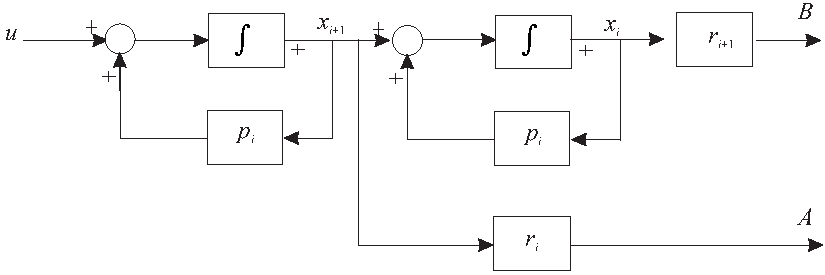
\includegraphics{pictures/jordanblock.pdf}}
\end{slide}
For this portion of the state space model we have
\begin{eqnarray*}
\left[\begin{array}{c}
  \dot{x}_i \\
  \dot{x}_{i+1}
\end{array}\right] &=& \left[\begin{array}{cc}
  p_i & 1 \\
  0 & p_i
\end{array}\right]\left[\begin{array}{c}
  x_i \\
  x_{i+1}
\end{array}\right] + \left[\begin{array}{c}
  0 \\
  1
\end{array}\right] u\\
y & = & \left[r_{i+1},\ r_i\right]\left[\begin{array}{c}
  x_i \\
  x_{i+1}
\end{array}\right].
\end{eqnarray*}

By comparison of this result with the normal situation we see that
the state matrices (of the observer controllable canonical form)
are modified as follows.
\begin{itemize}
  \item in $\mathbf{A}$ \[\left[\begin{array}{cc}
    p_i & 0 \\
    0 & p_{i+1} \\
  \end{array}\right] \rightarrow \left[\begin{array}{cc}
    p_i & 1 \\
    0 & p_{i} \\
  \end{array}\right];\]
  \item in $\mathbf{B}$ \[\left[\begin{array}{c}
    1 \\
    1  \\
  \end{array}\right] \rightarrow \left[\begin{array}{c}
    0 \\
    1 \\
  \end{array}\right];\]
    \item in $\mathbf{C}$ \[\left[\begin{array}{cc}
    r_i & r_{i+1}\\
  \end{array}\right] \rightarrow \left[\begin{array}{cc}
    r_{i+1} & r_i\\
  \end{array}\right].\]

\end{itemize}

The block \[\left[\begin{array}{cc}
    p_i & 1 \\
    0 & p_{i} \\
  \end{array}\right]\] is known as a ``\emph{Jordan Block}''. A
  matrix with one (or more) Jordan Blocks instead of a pure diagonal \[\left[\begin{array}{cc}
    p_i & 0 \\
    0 & p_{i+1} \\
  \end{array}\right]\] is in the ``\emph{Jordan Form}''. The idea
  may be extended to systems with poles of higher multiplicity.
  For example for the case where the multiplicity is 3 as in
  \[\frac{1}{(s-p_i)^3}\] the Jordan Block is  \[\left[\begin{array}{ccc}
    p_i & 1 & 0 \\
    0 & p_{i} & 1 \\
    0 & 0 & p_i
  \end{array}\right].\]

\subsection*{Example} The system with transfer function
\begin{eqnarray*}G(s) &=& \frac{1}{s^3 + 4s^2 + 5s + 2}\\
&=& \frac{1}{(s+1)^2(s+2)} \\ &=& \frac{-1}{s+1} +
\frac{1}{(s+1)^2} + \frac{1}{s+2}.\end{eqnarray*} The normal
canonical form is therefore given by:
\begin{eqnarray*}
\mathbf{A} &=& \left[\begin{array}{ccc}
  -1 & 1 & 0 \\
  0 & -1 & 0 \\
  0 & 0 & -2
\end{array}\right] \mathbf{B} = \left[\begin{array}{c}
  0 \\
  1 \\
  1
\end{array}\right]\\ \mathbf{C} &=& \left[\begin{array}{ccc}
  1 & -1 & 1
\end{array}\right] \mathbf{D} = \left[0\right]
\end{eqnarray*}

\subsection*{Normal Canonical Form with Complex Poles}
A system with complex poles will have a partial fraction expansion
containing terms of the form
\[\frac{\Re\{ r_i\} + j\Im\{ r_i\}}{s - \Re\{p_i\} + j\Im\{p_i\}} + \frac{\Re\{r_i\} - j\Im\{ r_i\}}{s - \Re\{p_i\} - j\Im\{p_i\}} \]
(where the poles and the residuals both appear as complex
conjugate pairs). We cannot implement these directly in state
space form because the state matrices must have real coefficients
to be realisable. However, the complex factors involved can be
combined into a quadratic form and blocks replaced in the normal
canonical form\footnote{The details are left as an exercise.} as
follows:
\begin{itemize}
  \item in $\mathbf{A}$ \[\left[\begin{array}{cc}
    p_i & 0 \\
    0 & p_{i+1} \\
  \end{array}\right] \rightarrow \left[\begin{array}{cc}
    +\Re\{p_i\} & +\Im\{p_i\} \\
    -\Im\{p_i\} & +\Re\{p_i\} \\
  \end{array}\right];\]
  \item in $\mathbf{B}$ \[\left[\begin{array}{c}
    1 \\
    1  \\
  \end{array}\right] \rightarrow \left[\begin{array}{c}
    0 \\
    1 \\
  \end{array}\right];\]
    \item in $\mathbf{C}$ \[\left[\begin{array}{cc}
    r_i & r_{i+1}\\
  \end{array}\right] \rightarrow \left[\begin{array}{cc}
    2\Im\{r_{i}\} & 2\Re\{r_i\}\\
  \end{array}\right].\]
\end{itemize}
\subsection*{Final Example}
 The system with transfer function
\begin{eqnarray*}G(s) &=& \frac{6s+6}{s^2 + 4s + 13}\\
&=& \frac{6(s+1)}{(s+2)^2 + 3^2} \\ &=&
\frac{6(s+1)}{(s+2+3j)(s+2-3j)}
\\ &=& \frac{3-j}{s+2+3j} + \frac{3-j}{s+2-3j}.\end{eqnarray*} The normal canonical form is
therefore given by:
\begin{eqnarray*}
\mathbf{A} &=& \left[\begin{array}{cc}
  -2-3j & 0 \\
  0 & -2+3j
\end{array}\right] \mathbf{B} = \left[\begin{array}{c}
  1 \\
  1
\end{array}\right]\\ \mathbf{C} &=& \left[\begin{array}{cc}
  3-j & 3+j
\end{array}\right] \mathbf{D} = \left[0\right]
\end{eqnarray*}
But this is not realisable so instead we use
\begin{eqnarray*}
\mathbf{A} &=& \left[\begin{array}{cc}
  -2 & -3 \\
  3 & -2
\end{array}\right] \mathbf{B} = \left[\begin{array}{c}
  0 \\
  1
\end{array}\right]\\ \mathbf{C} &=& \left[\begin{array}{cc}
  -2 & -6
\end{array}\right] \mathbf{D} = \left[0\right].
\end{eqnarray*}



%----------------------------------------------------------------
% The end of notes
% ----------------------------------------------------------------
\endinput

%%% Local Variables: 
%%% mode: latex
%%% TeX-master: t
%%% End: 
